\documentclass[]{article}
\usepackage{lmodern}
\usepackage{amssymb,amsmath}
\usepackage{ifxetex,ifluatex}
\usepackage{fixltx2e} % provides \textsubscript
\ifnum 0\ifxetex 1\fi\ifluatex 1\fi=0 % if pdftex
  \usepackage[T1]{fontenc}
  \usepackage[utf8]{inputenc}
\else % if luatex or xelatex
  \ifxetex
    \usepackage{mathspec}
  \else
    \usepackage{fontspec}
  \fi
  \defaultfontfeatures{Ligatures=TeX,Scale=MatchLowercase}
\fi
% use upquote if available, for straight quotes in verbatim environments
\IfFileExists{upquote.sty}{\usepackage{upquote}}{}
% use microtype if available
\IfFileExists{microtype.sty}{%
\usepackage{microtype}
\UseMicrotypeSet[protrusion]{basicmath} % disable protrusion for tt fonts
}{}
\usepackage[margin=1in]{geometry}
\usepackage{hyperref}
\hypersetup{unicode=true,
            pdftitle={Modulation of sensory behavior and food choice by an enteric bacteria-produced neurotransmitter},
            pdfauthor={Michael P. O'Donnell1,3, Bennett Fox2,Pin-Hao Chao1, Frank Schroeder2, and Piali Sengupta1,3},
            pdfborder={0 0 0},
            breaklinks=true}
\urlstyle{same}  % don't use monospace font for urls
\usepackage{graphicx,grffile}
\makeatletter
\def\maxwidth{\ifdim\Gin@nat@width>\linewidth\linewidth\else\Gin@nat@width\fi}
\def\maxheight{\ifdim\Gin@nat@height>\textheight\textheight\else\Gin@nat@height\fi}
\makeatother
% Scale images if necessary, so that they will not overflow the page
% margins by default, and it is still possible to overwrite the defaults
% using explicit options in \includegraphics[width, height, ...]{}
\setkeys{Gin}{width=\maxwidth,height=\maxheight,keepaspectratio}
\IfFileExists{parskip.sty}{%
\usepackage{parskip}
}{% else
\setlength{\parindent}{0pt}
\setlength{\parskip}{6pt plus 2pt minus 1pt}
}
\setlength{\emergencystretch}{3em}  % prevent overfull lines
\providecommand{\tightlist}{%
  \setlength{\itemsep}{0pt}\setlength{\parskip}{0pt}}
\setcounter{secnumdepth}{0}
% Redefines (sub)paragraphs to behave more like sections
\ifx\paragraph\undefined\else
\let\oldparagraph\paragraph
\renewcommand{\paragraph}[1]{\oldparagraph{#1}\mbox{}}
\fi
\ifx\subparagraph\undefined\else
\let\oldsubparagraph\subparagraph
\renewcommand{\subparagraph}[1]{\oldsubparagraph{#1}\mbox{}}
\fi

%%% Use protect on footnotes to avoid problems with footnotes in titles
\let\rmarkdownfootnote\footnote%
\def\footnote{\protect\rmarkdownfootnote}

%%% Change title format to be more compact
\usepackage{titling}

% Create subtitle command for use in maketitle
\providecommand{\subtitle}[1]{
  \posttitle{
    \begin{center}\large#1\end{center}
    }
}

\setlength{\droptitle}{-2em}

  \title{Modulation of sensory behavior and food choice by an enteric
bacteria-produced neurotransmitter}
    \pretitle{\vspace{\droptitle}\centering\huge}
  \posttitle{\par}
    \author{Michael P. O'Donnell\textsuperscript{1,3}, Bennett
Fox\textsuperscript{2},Pin-Hao Chao\textsuperscript{1}, Frank
Schroeder\textsuperscript{2}, and Piali Sengupta\textsuperscript{1,3}}
    \preauthor{\centering\large\emph}
  \postauthor{\par}
    \date{}
    \predate{}\postdate{}
  
\newcommand{\bcenter}{\begin{center}}
\newcommand{\ecenter}{\end{center}}

\begin{document}
\maketitle

\begin{center}

\textsuperscript{1}Department of Biology Brandeis University Waltham, MA
02454

\textsuperscript{2}Boyce Thompson Institute and Department of Chemistry
and Chemical Biology Cornell University Ithaca, NY 14850

\textsuperscript{3}Corresponding authors: M.O'D:
\href{mailto:mikeod@brandeis.edu}{\nolinkurl{mikeod@brandeis.edu}}; PS:
\href{mailto:sengupta@brandeis.edu}{\nolinkurl{sengupta@brandeis.edu}}

\hypertarget{running-title-sensory-neuromodulation-by-an-enteric-bacteria-produced-neurotransmitter}{%
\subsection{Running title: Sensory neuromodulation by an enteric
bacteria-produced
neurotransmitter}\label{running-title-sensory-neuromodulation-by-an-enteric-bacteria-produced-neurotransmitter}}

\end{center}

\hypertarget{animals-coexist-in-commensal-pathogenic-or-mutualistic-relationships-with-complex-communities-of-diverse-organisms-including-microbes1.-some-bacteria-produce-bioactive-neurotransmitters-which-have-been-proposed-to-modulate-host-nervous-system-activity-and-behaviors2.-however-the-mechanistic-basis-of-this-microbiota-brain-modulation-and-its-physiological-relevance-is-largely-unknown.-here-we-show-that-in-the-neuromodulator-tyramine-ta-produced-by-gut-colonizing-commensal-bacteria-can-bypass-the-requirement-for-host-biosynthesis-to-manipulate-a-host-sensory-decision.-bacterially-produced-ta-is-likely-converted-to-octopamine-oa-by-the-host-tyramine-beta-hydroxylase-enzyme.-oa-in-turn-targets-the-octr-1-receptor-on-the-ashasi-sensory-neurons-to-modulate-an-aversive-olfactory-response.-we-identify-genes-required-for-ta-biosynthesis-in-and-show-that-these-genes-are-necessary-for-modulation-of-host-behavior.-we-further-find-that-colonized-by-preferentially-select-these-bacteria-in-food-choice-assays-and-that-this-selection-bias-requires-bacterially-produced-ta.-our-results-demonstrate-that-a-neurotransmitter-produced-by-gut-microbiota-mimics-the-functions-of-the-cognate-host-biosynthetic-enzyme-to-override-host-control-of-a-sensory-decision-thereby-promoting-fitness-of-both-host-and-microbe.}{%
\subsubsection{\texorpdfstring{Animals coexist in commensal, pathogenic
or mutualistic relationships with complex communities of diverse
organisms including microbes1. Some bacteria produce bioactive
neurotransmitters which have been proposed to modulate host nervous
system activity and behaviors2. However, the mechanistic basis of this
microbiota-brain modulation and its physiological relevance is largely
unknown. Here we show that in \textit{C. elegans}, the neuromodulator
tyramine (TA) produced by gut-colonizing commensal \textit{Providencia}
bacteria can bypass the requirement for host biosynthesis to manipulate
a host sensory decision. Bacterially-produced TA is likely converted to
octopamine (OA) by the host tyramine beta-hydroxylase enzyme. OA in turn
targets the OCTR-1 receptor on the ASH/ASI sensory neurons to modulate
an aversive olfactory response. We identify genes required for TA
biosynthesis in \textit{Providencia}, and show that these genes are
necessary for modulation of host behavior. We further find that
\textit{C. elegans} colonized by \textit{Providencia} preferentially
select these bacteria in food choice assays, and that this selection
bias requires bacterially-produced TA. Our results demonstrate that a
neurotransmitter produced by gut microbiota mimics the functions of the
cognate host biosynthetic enzyme to override host control of a sensory
decision, thereby promoting fitness of both host and
microbe.}{Animals coexist in commensal, pathogenic or mutualistic relationships with complex communities of diverse organisms including microbes1. Some bacteria produce bioactive neurotransmitters which have been proposed to modulate host nervous system activity and behaviors2. However, the mechanistic basis of this microbiota-brain modulation and its physiological relevance is largely unknown. Here we show that in , the neuromodulator tyramine (TA) produced by gut-colonizing commensal  bacteria can bypass the requirement for host biosynthesis to manipulate a host sensory decision. Bacterially-produced TA is likely converted to octopamine (OA) by the host tyramine beta-hydroxylase enzyme. OA in turn targets the OCTR-1 receptor on the ASH/ASI sensory neurons to modulate an aversive olfactory response. We identify genes required for TA biosynthesis in , and show that these genes are necessary for modulation of host behavior. We further find that  colonized by  preferentially select these bacteria in food choice assays, and that this selection bias requires bacterially-produced TA. Our results demonstrate that a neurotransmitter produced by gut microbiota mimics the functions of the cognate host biosynthetic enzyme to override host control of a sensory decision, thereby promoting fitness of both host and microbe.}}\label{animals-coexist-in-commensal-pathogenic-or-mutualistic-relationships-with-complex-communities-of-diverse-organisms-including-microbes1.-some-bacteria-produce-bioactive-neurotransmitters-which-have-been-proposed-to-modulate-host-nervous-system-activity-and-behaviors2.-however-the-mechanistic-basis-of-this-microbiota-brain-modulation-and-its-physiological-relevance-is-largely-unknown.-here-we-show-that-in-the-neuromodulator-tyramine-ta-produced-by-gut-colonizing-commensal-bacteria-can-bypass-the-requirement-for-host-biosynthesis-to-manipulate-a-host-sensory-decision.-bacterially-produced-ta-is-likely-converted-to-octopamine-oa-by-the-host-tyramine-beta-hydroxylase-enzyme.-oa-in-turn-targets-the-octr-1-receptor-on-the-ashasi-sensory-neurons-to-modulate-an-aversive-olfactory-response.-we-identify-genes-required-for-ta-biosynthesis-in-and-show-that-these-genes-are-necessary-for-modulation-of-host-behavior.-we-further-find-that-colonized-by-preferentially-select-these-bacteria-in-food-choice-assays-and-that-this-selection-bias-requires-bacterially-produced-ta.-our-results-demonstrate-that-a-neurotransmitter-produced-by-gut-microbiota-mimics-the-functions-of-the-cognate-host-biosynthetic-enzyme-to-override-host-control-of-a-sensory-decision-thereby-promoting-fitness-of-both-host-and-microbe.}}

The pathways mediating chemical communication between colonizing gut
bacteria and the host nervous system are largely undescribed2. Recently,
the nematode \textit{C. elegans} has emerged as a powerful system in
which to study host-microbe chemical communication3, offering an
opportunity to experimentally address how microbiota influence host
nervous system function. In the wild, diverse populations of pathogenic
and non-pathogenic bacteria colonize the \textit{C. elegans} intestine
and serve as the primary food source for this nematode4. Exposure to
pathogenic bacteria alters \textit{C. elegans} olfactory behaviors5, but
whether commensal gut bacteria also modulate host behaviors is unknown4.

To identify novel modes of microbial influences on host sensory
behaviors, we screened non-pathogenic bacterial strains typically
associated with wild nematodes6 for their ability to influence
\textit{C. elegans} olfactory responses. In long-range chemotaxis
assays7, adult hermaphrodites co-cultivated on these bacterial strains
exhibited robust attraction to a panel of attractive volatile odorants
similar to the behaviors of animals grown on the standard
\textit{E. coli} food source OP50 (Fig. 1a). However, co-cultivation
with the \textit{Providencia} alcalifaciens strain (JUb39)6,8 resulted
in decreased avoidance of 100\% 1-octanol as compared to OP50-grown
animals (Fig. 1b; this decreased avoidance is henceforth referred to as
octanol modulation). Avoidance of the volatile and osmotic repellents
2-nonanone and 8M glycerol, respectively, was unaffected upon growth on
JUb39 (Fig. 1b, Extended Data Fig. 1a), suggesting that JUb39 modulates
responses of \textit{C. elegans} to a selective subset of nociceptive
chemical stimuli. Animals grown on a distantly related
\textit{Providencia} rettgeri strain isolated from nematodes in compost
(PYb007, Extended Data Fig. 1b) exhibited similar octanol modulation
(Fig. 1c). These observations indicate that upon co-culture, multiple
\textit{Providencia} strains modulate octanol aversion in
\textit{C. elegans}.

\begin{center}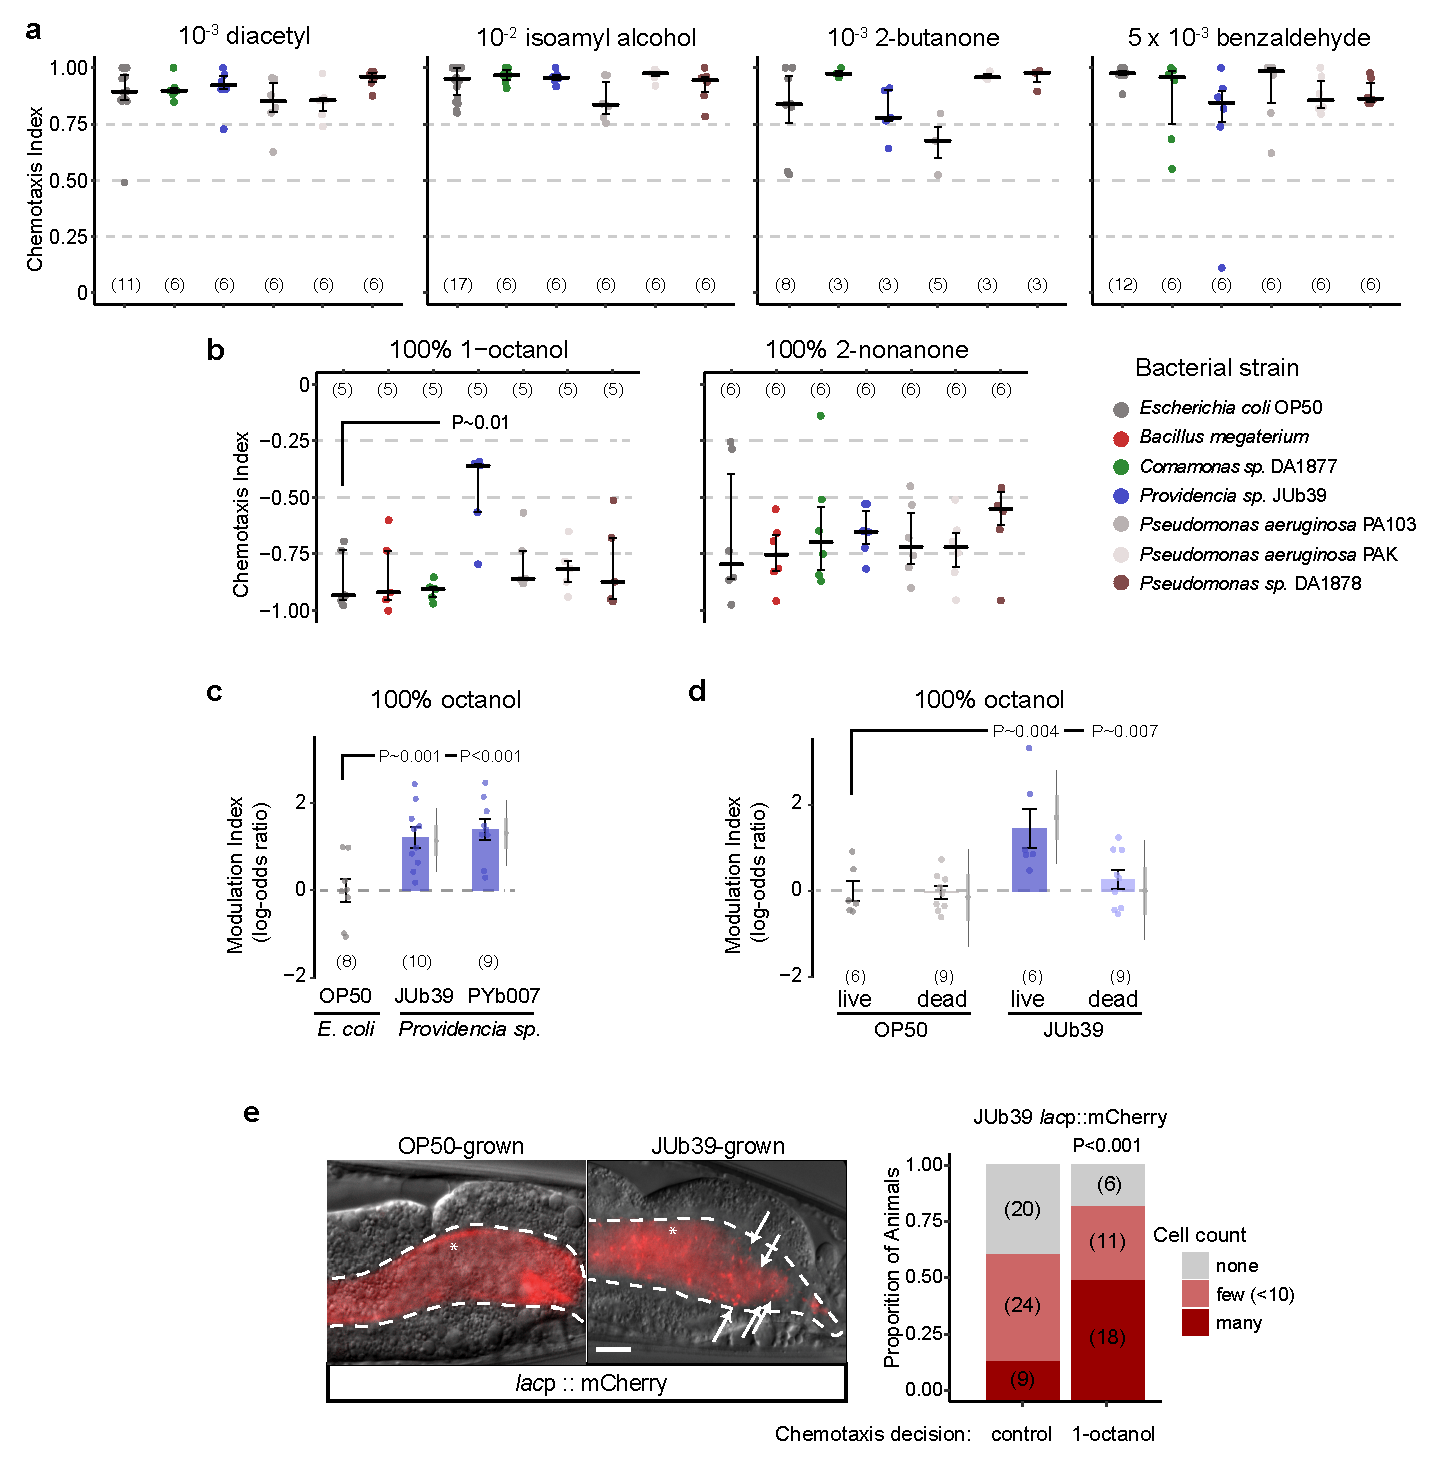
\includegraphics[width=0.75\linewidth]{Figure_1v5} \end{center}

\begin{itemize}
  \item[] Fig. 1. \textit{Providencia} colonizes the \textit{C. elegans} intestine and modulates octanol avoidance behavior.
a-b) Long-range chemotaxis assays to attractive (a) or aversive (b) odors of \textit{C. elegans} grown on the indicated bacterial strains. Chemotaxis index (CI) = (animals at the odorant – animals at the control)/total number of animals. Each dot indicates the CI from a single assay of approximately 100 animals. Positive and negative numbers indicate attraction and avoidance, respectively. Horizontal line is median; errors are 1st and 3rd quartiles. P-value indicated is from a binomial general linearized mixed-effects model (GLMM) with random intercepts for assay plate and date and with false discovery rate (FDR) for post-hoc comparisons. Numbers in parentheses indicate total number of assays.
c-d) Modulation index of worms grown on the indicated bacterial strains (c) or bacterial strains pre-treated with 200 \(\mu\)g/\(\mu\)L gentamicin for 2 hrs prior to plating (d) in response to 100% octanol. Modulation index is defined as the log odds-ratio of the proportion of worms at octanol vs control of each condition relative to the OP50-grown condition per independent day. Modulation index values are shown on a log-odds (logit) scale and are normalized to the values of wild-type animals grown on OP50 for each day, indicated with a gray dashed line. Positive numbers indicate reduced octanol avoidance. Errors are SEM. Gray thin and thick vertical bars at right indicate Bayesian 95% and 66% credible intervals, respectively. P-values between the indicated conditions are from a GLMM with Dunnett-type multivariate-t adjustment for c, and Tukey-type multivariate-t adjustment for d. 
e) Presence of mCherry-expressing bacteria in the posterior intestines of young adult animals indicated with micrographs (left) or quantified (right). Arrows in micrographs indicate intact rod-shaped cells, asterisk indicates diffuse intestinal fluorescence. Dashed line in micrographs indicate the intestinal boundary. Anterior is at left. Scale bar: XXXX. Bars at right show proportion of animals with the indicated distribution of JUb39 cells present in animals that migrated to 100% octanol or the control in chemotaxis assays. Numbers in parentheses indicate the number of animals; 3 independent assays. P-value is derived from an ordinal regression.
\end{itemize}

Under specific conditions, food deprivation reduces octanol avoidance9.
JUb39 has been categorized as a `beneficial' bacterium that supports
robust \textit{C. elegans} growth and does not induce stress responses6,
suggesting that JUb39-fed animals are unlikely to be nutrition-deprived.
In support of this notion, growth on JUb39 did not alter expression of a
tph-1p::gfp fusion gene, a reporter of feeding state10,11 (Extended Data
Fig. 1c). Moreover, growth of \textit{C. elegans} on the poor bacterial
food Bacillus megaterium12 did not alter octanol avoidance (Fig. 1b). We
infer that the observed octanol modulation by \textit{Providencia} is
unlikely to be solely due to changes in feeding state.

While OP50 is typically crushed by the pharyngeal grinder in young adult
\textit{C. elegans}13, a subset of bacterial strains can bypass the
grinder and survive in the worm intestine6,14,15. We found that feeding
\textit{C. elegans} with JUb39 pre-treated with high concentrations of
the antibiotic gentamicin eliminated octanol modulation (Fig. 1d),
indicating that JUb39 must be alive to mediate this behavioral
plasticity. In addition, neither exposure of OP50-grown animals to
JUb39-derived odors nor pre-incubation of OP50-grown animals with
JUb39-conditioned media was sufficient to result in octanol modulation
(Extended Data Fig. 1e), further suggesting that \textit{C. elegans}
must ingest live JUb39 to induce octanol modulation.

To test whether colonization of the worm gut drives octanol modulation,
we transformed OP50 and JUb39 with a plasmid encoding a constitutively
expressed mCherry fluorescent reporter. While the guts of OP50-fed adult
worms displayed only diffuse intestinal fluorescence consistent with
these bacteria being lysed, the guts of JUb39-fed worms contained
variable but typically large numbers of intact rod-shaped cells
expressing mCherry (Fig. 1e), likely indicating the presence of live
JUb39. These cells tended to be enriched in the posterior intestine
(Fig. 1e), unlike the reported localization pattern of severely
pathogenic bacteria16. Moreover, nematodes colonized by JUb39 did not
exhibit phenotypes characteristic of pathogenic infection such as anal
swelling17 (Fig. 1e), further confirming that JUb39 is largely
non-pathogenic to \textit{C. elegans}. We next performed chemotaxis
assays with animals fed on mCherry-labeled JUb39, and quantified
intestinal bacterial cells in animals that had navigated either toward
octanol or toward the control. We found that animals navigating toward
octanol consistently contained more gut bacteria (Fig. 1e). We conclude
that JUb39 colonizes the worm gut and the extent of colonization is
correlated with decision-making in response to octanol.

We investigated the mechanistic basis for \textit{Providencia}-mediated
octanol modulation. Octanol avoidance is subject to extensive modulation
directly and indirectly via multiple biogenic amines including tyramine
(TA) and octopamine (OA) (Fig. 2a) as well as neuropeptides9,18-22. TA
is produced from Tyrosine (L-Tyr) via the activity of a tyrosine
decarboxylase (TDC; encoded by tdc-1 in \textit{C. elegans}); TA is
subsequently converted to OA via a tyramine beta hydroxylase (encoded by
tbh-1)23 (Fig. 2a). Consequently, all tbh-1 mutant phenotypes resulting
from lack of OA are expected to be shared by tdc-1 mutants23.
Surprisingly, we found that while tdc-1 mutants grown on JUb39 continued
to exhibit octanol modulation, the modulation exhibited by tbh-1 mutants
was significantly reduced (Fig. 2b). Mutations in the cat-2 tyrosine
hydroxylase24 and tph-1 tryptophan hydroxylase25 enzymes required for
the production of biogenic amines dopamine and serotonin in
\textit{C. elegans}, respectively, did not affect octanol modulation
(Fig. 2b). These results raise the possibility that
\textit{C. elegans}-produced OA, but not TA, is partly necessary for
JUb39-mediated octanol modulation.

\begin{center}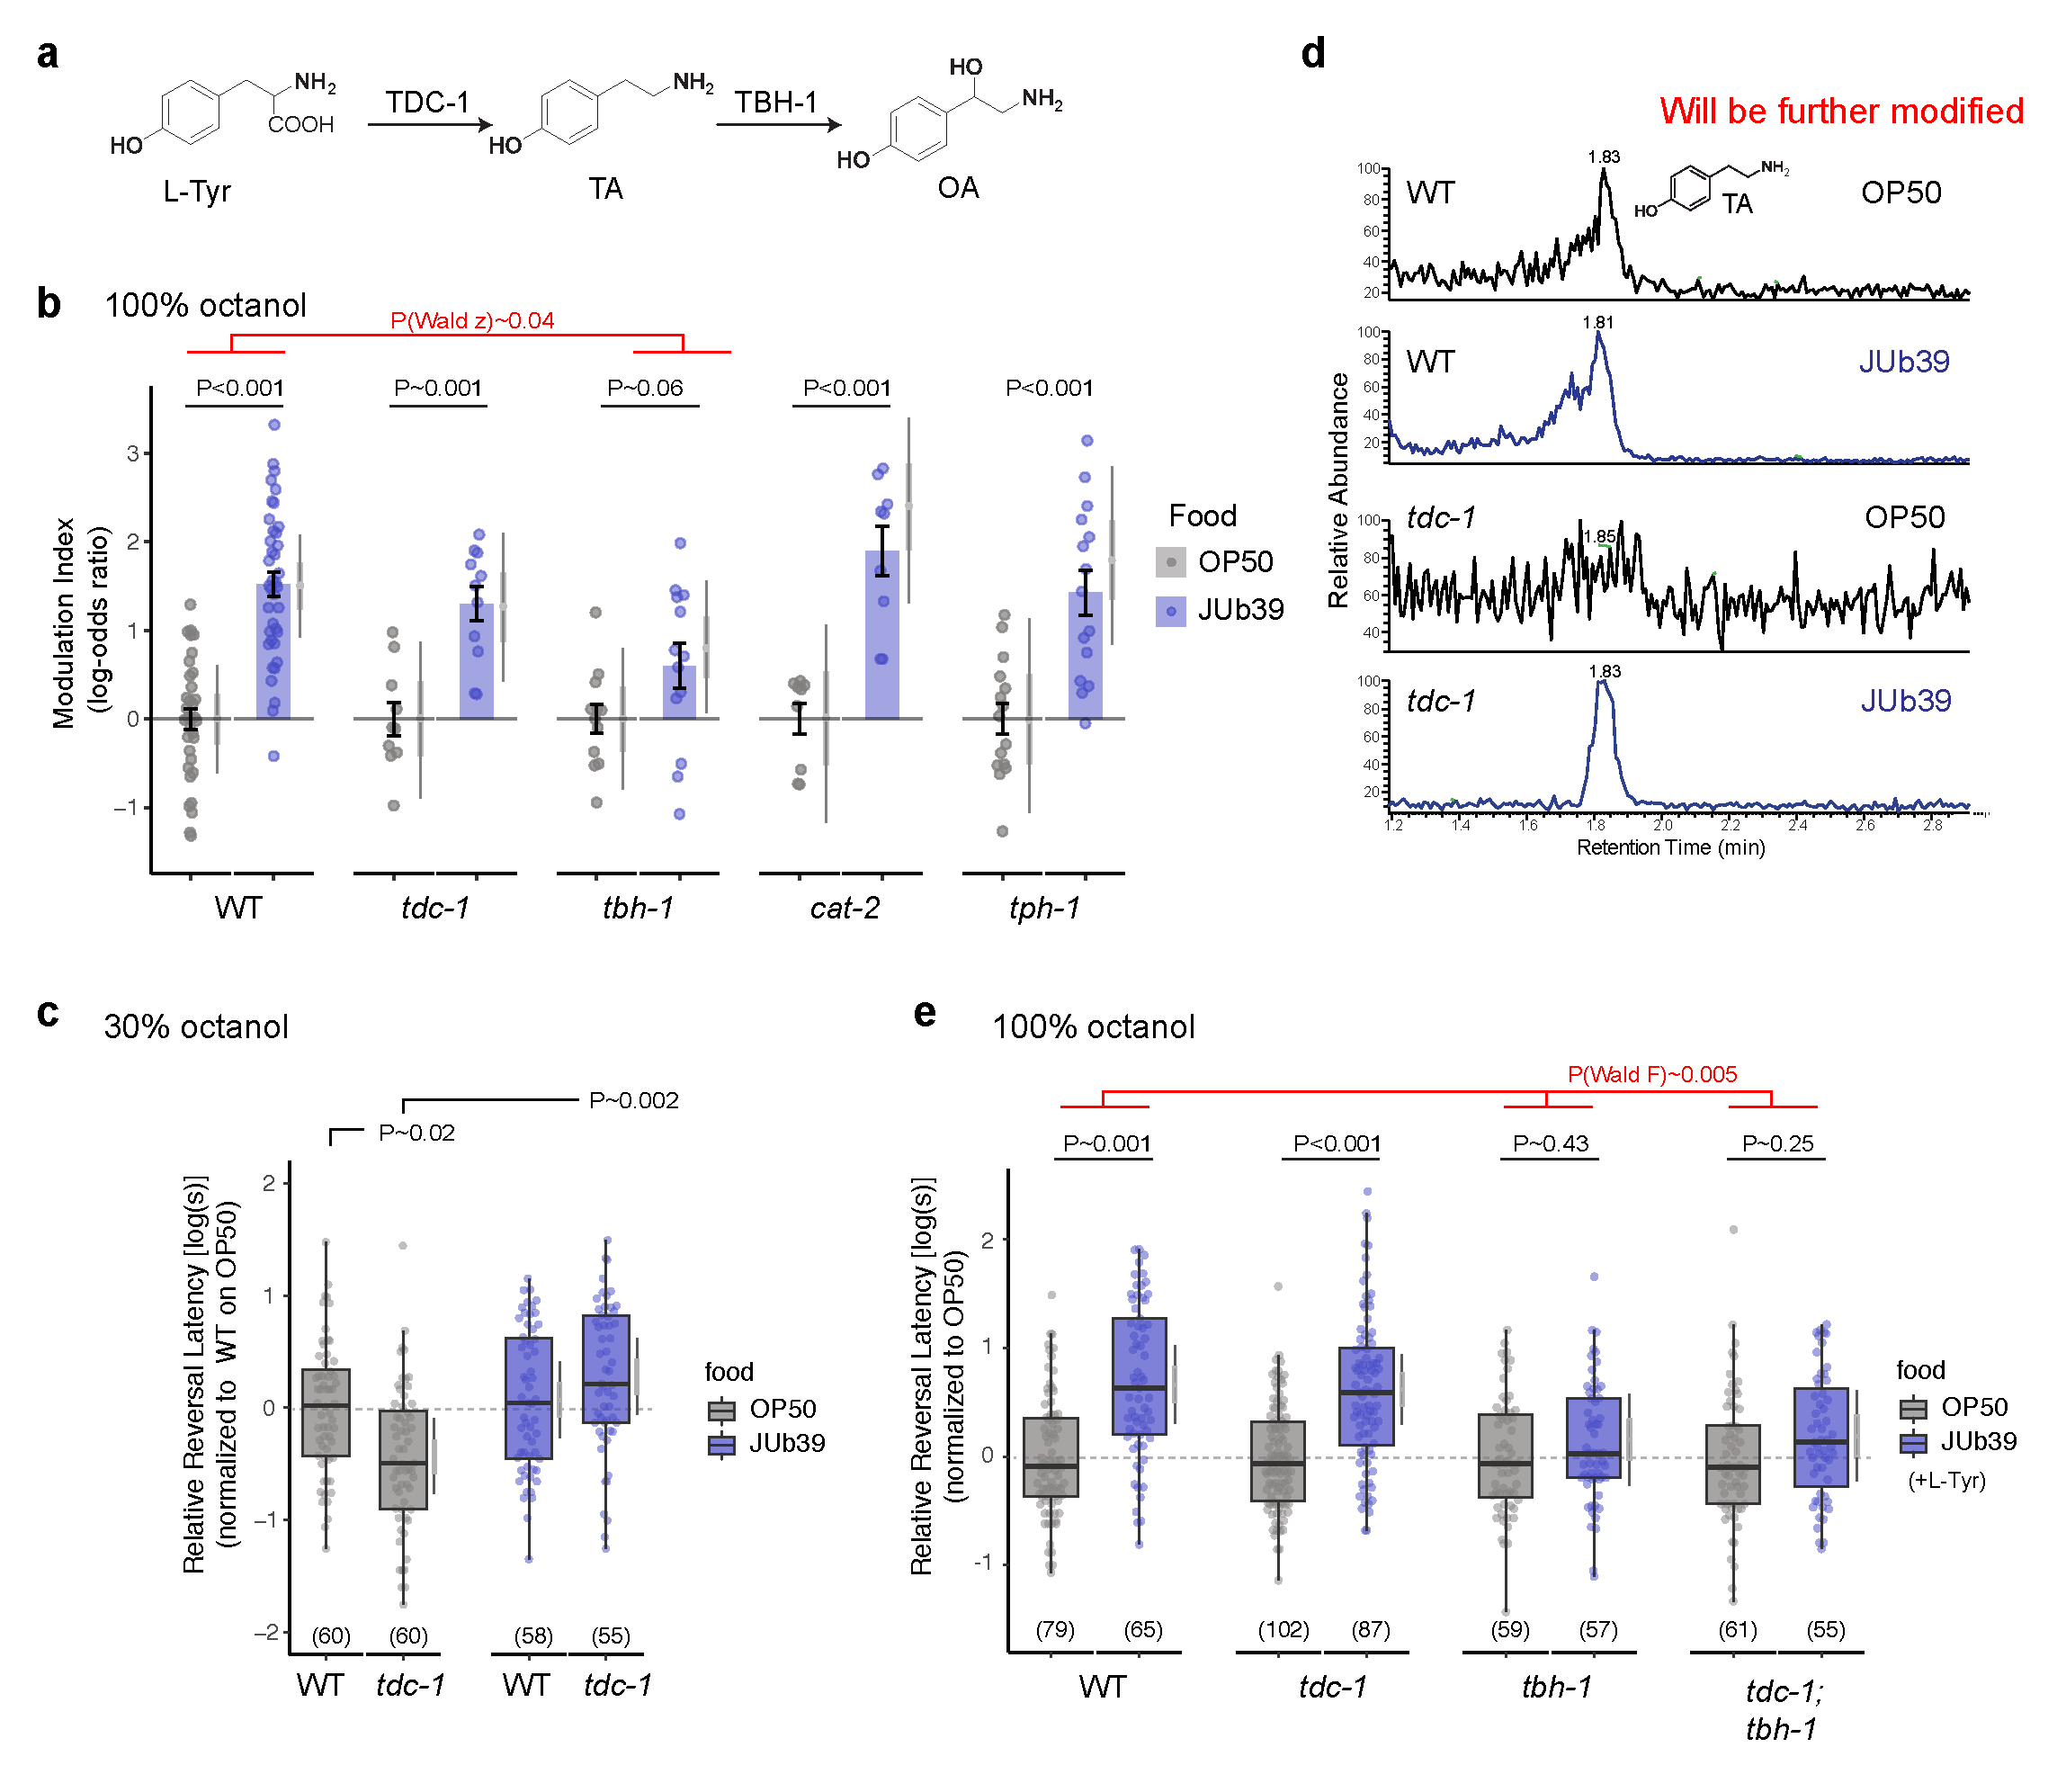
\includegraphics[width=0.75\linewidth]{Figure_2vB6} \end{center}

\begin{itemize}
  \item[] Fig. 2. \textit{Providencia} produces TA which compensates for loss of \textit{C. elegans} tdc-1. 
a) Biosynthesis pathway of TA and OA from L-Tyr in \textit{C. elegans}23. b) Modulation index of worms of the indicated genotypes grown on OP50 or JUb39 in response to 100% octanol. Each dot represents results from one chemotaxis assay with approximately n animals each. Values are shown on the log-odds (logit) scale and are normalized to the values of animals of the corresponding genotypes grown on OP50 for each day, indicated with gray dashed lines. Positive numbers indicate reduced avoidance of octanol. Errors are SEM. Gray thin and thick vertical bars at right indicate Bayesian 95% and 66% credible intervals, respectively. P-values between the indicated conditions are from a GLMM with Dunnett-type multivariate-t adjustment. P-value in red indicates Wald z-statistic for the magnitude of the JUb39 effect in tbh-1 compared to wild-type. c, e) Reversal response latency of animals of the indicated genotypes grown on OP50 or JUb39 on NGM (c) or NGM + 0.5% L-Tyr (e) in response to 30% octanol (c) or 100% octanol (e) in SOS assays. Each dot is the response time of a single animal. The Y-axis is log10-scaled for these log-normal distributed data, and normalized to the indicated control group for each experimental day. Numbers in parentheses indicate the number of worms tested in assays over at least 3 independent days. Boxplot indicates median and quartiles, whiskers indicate the data range, excluding outliers. Gray thin and thick vertical bars at right indicate Bayesian 95% and 66% credible intervals for the difference of means, respectively. P-values between the indicated conditions are from a linear-mixed effects regression on log-transformed data (LMM). P-value in red (e) indicates Wald F-statistic for the effect of the indicated genotypes on the magnitude of the JUb39 effect. d) High resolution LC-MS analysis of animals of the indicated genotypes grown on the indicated bacterial strains. 
\end{itemize}

To account for these observations, we hypothesized that JUb39 produces
TA that may functionally compensate for the host tdc-1 mutation. tdc-1
mutants grown on OP50 have been reported to display more rapid aversive
responses to dilute (30\%) octanol18. Exogenous TA suppresses this
increased aversion of tdc-1 animals but does not alter wild-type
responses under the same conditions18. To test if JUb39 is able to
suppress behavioral defects of tdc-1 mutants, we performed short-range
acute avoidance assays {[}the ``smell-on-a-stick'' (SOS) assay{]}9,26.
In this assay, the strength of avoidance is inversely correlated with
reversal latency when the animal encounters the repellent as it is
moving forward. As expected, tdc-1 mutants grown on OP50 responded more
rapidly to 30\% octanol than wild-type animals. This enhanced aversion
was suppressed upon growth on JUb39 (Fig. 2c). These results are
consistent with the notion that bacterially-produced TA functionally
complements for the loss of host-derived TA in driving a sensory
behavioral decision.

To directly test for the production of TA by JUb39, we measured TA
levels using high-resolution HPLC-MS of wild-type and tdc-1 mutant adult
worms grown on either OP50 or JUb39. We focused on a TA derivative,
N-succinyl-tyramine, as a proxy for TA because this chemical is present
at higher levels than free TA under these conditions27. While
N-succinyl-tyramine was present in wild-type animals regardless of the
food source, this chemical was not detected in tdc-1 mutants grown on
OP5023. However, N-succinyl-tyramine was restored upon growth of tdc-1
mutants on JUb39 (Fig. 2d). OA was undetectable under these conditions
in both WT and tdc-1 mutants. We conclude that JUb39 in association with
\textit{C. elegans} produces TA which can accumulate in the host.

Although TA biosynthesis in bacteria has been demonstrated in some
gram-positive genera, production appears to be uncommon in gram-negative
bacteria which include \textit{Providencia}28,29. TA production in
gram-positive strains is induced upon supplementation with L-Tyr30. We
found that growth on L-Tyr-supplemented media enhanced octanol
modulation by JUb39 in SOS assays (Extended Fig. 2). Under these
conditions, mutations in tbh-1 fully suppressed octanol modulation in
SOS assays, while as observed in long-range chemotaxis assays, tdc-1
mutants continued to exhibit robust octanol modulation (Fig. 2e).
Octanol avoidance behaviors of tdc-1; tbh-1 double mutants were similar
to those of tbh-1 mutants alone (Fig. 2e), indicating that the lack of
host-derived OA, and not accumulation of TA due to loss of TBH-123,27
accounts for the reduced octanol modulation in tbh-1 mutants.

Biogenic amines are typically generated from aromatic amino acids and
L-glutamate by pyridoxyl phosphate (PLP)-dependent group II aromatic
acid decarboxylase enzymes (AADCs) in both eukaryotes and bacteria31
(Extended Data Fig. 3a-b, Extended Data Table 1). In gram-positive
Enterococcus and Lactobacillus (Lb), TA production is mediated by the
TDC-encoding (\textit{tyrDC}) AADC and tyrosine permease/transporter
(tyrP) genes present in an operon; this operon is inducible by L-Tyr
(Fig. 3a-b, Extended Fig. 3a-b, Extended Data Table 1)32,33. Although
genes related to Enterococcus \textit{tyrDC} and tyrP were largely
absent in Gammaproteobacteria (Fig. 3b), we confirmed the presence of
homologous operons containing \textit{tyrDC} and tyrP in JUb39 and
PYb007 de novo genome assemblies via whole genome sequencing (Fig. 3a,
Extended Data Fig. 3b, Extended Data Table 1). \textit{tyrDC} homologs
were also identified in the genomes of additional members of the
Morganellaceae family, although the operon structure was conserved in
only a subset of these genomes (Fig. 3a, Fig. 3c, Extended Fig. 3b,
Extended Data Table 1).

\textit{Providencia} TyrDC is highly homologous to the Lb enzyme, which
has been well characterized with respect to substrate specificity34.
Protein modeling using the crystal structure of Lb-TyrDC34 as a guide
(see Methods) indicated that JUb39 TyrDC shares most known catalytic
sites with Lb-TyrDC (Fig. 3d). Interestingly, JUb39 TyrDC contains a
substitution at A600 (S586 in Lb-TyrDC; Fig.3d), a variant demonstrated
to enhance specific catalytic activity of Lb-TyrDC for tyrosine34. We
infer that JUb39 TyrDC likely generates TA from tyrosine.

Morganella strains (Morganellaceae family) have been reported to produce
TA under certain conditions28, despite having no discernible
\textit{tyrDC} orthologs (Fig. 3c, Extended Data Fig. 3c, Extended Data
Table 1). Instead in Morganella, we identified an AADC-encoding gene
(hereafter \textit{adcA}) with \textasciitilde{}29\% and 27\% sequence
identity to Enterococcus TyrDC and human GAD67, respectively, in an
operon upstream of a gene encoding a TYT-1 family tyrosine permease
(Fig. 3a, Fig. 3c). An \textit{adcA} homolog is also present in
\textit{Providencia} genomes including in JUb39 but is not adjacent to a
tyrosine transporter (Fig. 3b-c, Extended Data Fig. 3a-b, Extended Data
Table 1). We conclude that \textit{Providencia} encodes at least two
AADCs with the potential to generate TA, and the phylogenetic
incongruence suggests that both \textit{tyrDC} and \textit{adcA} genes
may have either been lost or acquired in the Morganellaceae family via
horizontal gene transfer.

To test whether one or both JUb39 AADCs are necessary for octanol
modulation, we engineered deletions in JUb39 \textit{tyrDC} and
\textit{adcA} (\(\Delta\)\textit{tyrDC}::cmR and
\(\Delta\)\textit{adcA}, respectively; Fig. 3a). While cultivation on
each deletion-containing bacterial strain alone weakly decreased octanol
modulation, growth on the JUb39 \(\Delta\)\textit{tyrDC}::cmR
\(\Delta\)\textit{adcA} double knockout bacteria abolished octanol
modulation (Fig. 3e). We confirmed that JUb39
\(\Delta\)\textit{tyrDC}::cmR \(\Delta\)\textit{adcA} colonizes the
\textit{C. elegans} gut but fails to produce TA derivatives (Extended
Data Fig. 4a-b). Octanol modulation was restored upon growth of
wild-type \textit{C. elegans} on JUb39 \(\Delta\)\textit{tyrDC}::cmR
\(\Delta\)\textit{adcA} strains supplemented with TA on agar plates
(Fig. 3f). Moreover, while exogenous TA did not further increase octanol
avoidance in wild-type JUb39-grown animals, TA supplementation resulted
in octanol modulation in OP50-grown animals (Fig. 3f). Together, these
results indicate that TA produced by multiple AADC enzymes in
\textit{Providencia} is both necessary and sufficient to modulate
octanol avoidance by wild-type \textit{C. elegans}.

We next identified the molecular targets of
\textit{Providencia}-mediated octanol modulation in the host. As
bacterially-produced TA is likely converted to OA via the host TBH-1
enzyme23 to mediate octanol modulation, we focused primarily on host OA
receptors. The bilateral ASH nociceptive neurons located in the head
amphid organs of \textit{C. elegans} have been implicated in sensing
octanol9,19,26. These neurons express multiple TA and OA receptors, a
subset of which is required for octanol modulation by these
monoamines18,35. Among ASH-expressed OA receptors, mutations in octr-1,
but not ser-3, abolished JUb39-mediated octanol modulation, without
altering the extent of gut colonization (Fig. 4a, Extended Data Fig.
4b). We also observed an effect on octanol modulation in tyra-2 TA
receptor mutants, which were recently shown to interfere with detection
of OA-linked pheromones36. This was primarily due to decreased octanol
avoidance upon growth on OP50 (4.3 ± 0.25s for tyra-2 vs.~2.9 ± 0.13s
for WT); the reason for this phenotype is currently unclear. Expression
of octr-1 cDNA in the ASH/ASI sensory neurons restored octanol
modulation (Fig. 4a). octr-1 mutants also lacked octanol modulation when
grown on JUb39 \(\Delta\)\textit{tyrDC}::cmR \(\Delta\)\textit{adcA}
supplemented with TA (Fig. 4b). We conclude that host OA produced upon
JUb39 colonization acts via OCTR-1 in ASH/ASI to modulate octanol
avoidance.

Next we investigated the biological relevance of the JUb39-directed
decrease in octanol aversion by \textit{C. elegans}. While many
gram-negative enteric bacteria produce long-chain alcohols including
octanol37, whether \textit{Providencia} produces this chemical is
unknown. However, JUb39 and other \textit{Providencia} strains can
produce the branched alcohol isoamyl alcohol (IAA), which is aversive to
\textit{C. elegans} when concentrated38,39. Similar to octanol,
avoidance of high IAA concentrations is also mediated by the ASH sensory
neurons39. We hypothesized that reduced avoidance of JUb39-produced
aversive alcohols may preferentially bias JUb39-grown
\textit{C. elegans} to select these bacteria in food choice assays.
Indeed, animals grown on JUb39 more strongly preferred JUb39 compared to
OP50-grown worms, which showed a slight preference for JUb39 in a
short-range food choice assay (Fig. 4c). The bias towards JUb39 was
eliminated in animals grown on JUb39 \(\Delta\)\textit{tyrDC}::cmR
\(\Delta\)\textit{adcA}, suggesting that bacterial TA production is
necessary for this food preference (Fig 4b). Together, these results
imply that TA produced by JUb39 reduces ASH/ASI-mediated avoidance of
JUb39-produced aversive cues such as concentrated alcohols, to allow
preferential selection of these bacteria.

Our observations support a model in which the neurotransmitter TA
produced by intestinal \textit{Providencia} bacteria modulates aversive
responses of \textit{C. elegans} to the enteric bacteria-produced
volatile metabolite octanol, likely via subverting host-dependent TA
production. Bacterially produced TA is converted to OA by
\textit{C. elegans} TBH-1; OA subsequently acts on the ASH/ASI neurons
via the OCTR-1 OA receptor to increase the preference of
\textit{C. elegans} for \textit{Providencia} in food choice assays (Fig.
4d). We speculate that the preference for \textit{Providencia} upon
colonization of \textit{C. elegans} by these bacteria promotes increased
consumption leading to stable association4,40 and bacterial dispersal.
As \textit{Providencia} is a rich food source for \textit{C. elegans}6,
this association may be mutually beneficial. Our results describe a
pathway by which neurotransmitters produced by commensal bacterial
direct host behavioral decisions by supplementing or compensating for
the activity of key host biosynthetic enzymes, thereby altering fitness
of both host and microbe.

\hypertarget{figure-legends}{%
\section{FIGURE LEGENDS}\label{figure-legends}}

Fig. 3. Two amino acid decarboxylase enzymes encoded by the
\textit{Providencia} genome act redundantly to modulate octanol
avoidance. a) Cartoons depicting the \textit{tyrDC} locus (top) in
Lactobacillales (left) and JUb39 (right) and the \textit{adcA} locus
(bottom) in Morganella (left) and JUb39 (right). b) Presence of
\textit{tyrDC} and \textit{adcA} among complete genomes in
Gammaproteobacteria. Linked boxes indicate organization in an operon.
Hatched shading indicates variable presence among genera. Colored
triangles indicate taxa of interest. c) Presence of \textit{tyrDC},
\textit{adcA}, E.coli-type tyrP and Morganella-type tyt-1 at the family
and genus level among Enterobacteriales. Linked boxes indicate
organization in an operon. d) Homology-based model of the TyrDC
catalytic domain in \textit{Providencia} based on the Lb-TyrDC crystal
structure34 using SWISS-MODEL (\url{https://swissmodel.expasy.org}).
Residues in magenta, green and yellow are from Lb-TyrDC, JUb39-TyrDC,
and JUb39-AdcA, respectively. PLP is depicted in red and L-Tyr (manually
docked for illustration) is indicated in light blue. Position of
A600/S58634 in JUb39 TyrDC and Lb-TyrDC are indicated. e-f) Reversal
response times of animals of wild-type \textit{C. elegans} grown on the
indicated bacterial genotypes in either control conditions of NGM +
0.5\% L-Tyr (e) or supplemented with the indicated concentrations of TA
(f) to 100\% octanol using SOS assays. Each dot is the response time of
a single worm. Y-axis is log10-scaled for these log-normal distributed
data, and normalized to the indicated control group for each
experimental day. Numbers in parentheses indicate the number of worms
tested in assays over at least 3 independent days. Boxplot indicates
median and quartiles, whiskers indicate the data range, excluding
outliers. Gray thin and thick vertical bars at right indicate Bayesian
95\% and 66\% credible intervals for the difference of means,
respectively. P-values between indicated conditions are from a LMM with
Tukey-type multivariate-t adjustment).

Fig. 4. Modulation of octanol avoidance by \textit{Providencia} requires
the OCTR-1 OA receptor in the ASH/ASI sensory neurons. a-b) Reversal
response times of animals of the indicated genotypes grown on the shown
bacteria in control conditions of NGM + 0.5\% L-Tyr (a) or supplemented
with TA + 0.5\% L-Tyr (b) to 100\% octanol using SOS assays. Each dot is
the response time of a single worm. Y-axis is log10-scaled for these
log-normal distributed data, and normalized to the indicated control
group for each experimental day. Numbers in parentheses indicate the
number of worms tested in assays over at least 3 independent days.
Boxplot indicates median and quartiles, whiskers indicate the data
range, excluding outliers. Gray thin and thick vertical bars at right
indicate Bayesian 95\% and 66\% credible intervals for the difference of
means, respectively. P-values between indicated conditions are from a
LMM with Tukey-type multivariate-t adjustment. c) (Left) Cartoon
depicting assay setup of the short-range bacterial choice assay. (Right)
Preference index of animals grown on the indicated bacteria for the test
bacteria JUb39. Each dot represents one assay of at least 10 animals
over at least 4 independent days. Y-axis is on log-odds (logit) scale.
Errors are SEM. Gray thin and thick vertical bars at right indicate
Bayesian 95\% and 66\% credible intervals, respectively. P-values
represent difference of means relative to JUb39-grown animals from a
GLMM with Dunnett-type multivariate-t adjustment. d) Cartoon of working
model. JUb39 colonizes the \textit{C. elegans} intestine and produces TA
via the TyrDC and \textit{adcA} enzymes. TA is converted to OA by
\textit{C. elegans} TBH-1 and acts via the ASH neuron-expressed OCTR-1
OA receptor to modulate octanol avoidance and food choice.

Extended Data Fig. 1. Octanol modulation by \textit{Providencia}
requires ingestion of bacteria but is not mediated by nutritive cues.\\
a) Osmotic ring avoidance assays. Each dot represents one assay of 10
animals. Numbers in parentheses indicate the number of assays over at
least 3 independent days. Y-axis is proportion of animals leaving an
osmotic ring barrier of 8M glycerol after 10 minutes. P-value represents
difference of means relative to JUb39-grown animals from a GLMM. Errors
are SEM. Gray thin and thick vertical bars at right indicate Bayesian
95\% and 66\% credible intervals, respectively. b) Isolation of
nematode-associated bacteria. Nematodes were isolated from residential
compost in Massachusetts. Worms were allowed to crawl onto NGM plates
from which they were picked to clean plates. Resulting bacterial
colonies were isolated, grown on LB media and characterized via 16S rRNA
sequencing. c) Expression of a tph-1p::gfp fluorescent reporter in
indicated head neurons of young adult animals grown on either OP50 or
JUb39. Each dot is the mean fluorescence of the soma of one neuron.
Horizontal bar is mean; errors are SEM. Gray thin and thick vertical
bars at right indicate Bayesian 95\% and 66\% credible intervals,
respectively. P-values are from two-way ANOVA. d-e) Modulation index of
worms grown on the indicated bacterial strains, under the shown
conditions. Animals were exposed to the indicated bacteria on the plate
lid (d) for one generation, or to NGM control or bacteria-conditioned
NGM (e) for 2 hours prior to the assay. Each dot represents results from
one chemotaxis assay with approximately 100 animals each. Values are
shown on a log-odds (logit) scale and are normalized to the values of
wild-type animals grown on OP50 for each day, indicated with a gray
dashed line. Positive numbers indicate reduced avoidance of octanol.
Errors are SEM. Gray thin and thick vertical bars at right indicate
Bayesian 95\% and 66\% credible intervals, respectively. P-values
between the indicated conditions are post-hoc comparisons from a GLMM,
with Tukey-type multivariate-t adjustment for e.

Extended Data Fig. 2. L-Tyr supplementation enhances octanol modulation.
Reversal response times of animals of the indicated genotypes grown on
the indicated bacteria in control conditions or supplemented with 0.5\%
L-Tyr to 100\% octanol using SOS assays. Each dot is the response time
of a single worm. Y-axis is log10-scaled for these log-normal
distributed data, and normalized to the indicated control group for each
experimental day. Numbers in parentheses indicate the number of worms
tested in assays over at least 3 independent days. Boxplot indicates
median and quartiles, whiskers indicate the data range, excluding
outliers. Gray thin and thick vertical bars at right indicate Bayesian
95\% and 66\% credible intervals for the difference of means,
respectively. P-values indicating comparisons of means relative to the
OP50 control for each conditions are from a LMM with Tukey-type
multivariate-t adjustment. P-value in red indicates Wald F-statistic for
the effect of L-Tyr supplementation on the magnitude of the JUb39
effect.

Extended Data Fig. 3. Phylogenetic analysis of group II decarboxylase
genes in Gammaproteobacteria. a) Neighbor-joining unrooted tree based on
sequences identified via a BLAST search using Enterococcus faecalis
TyrDC and \textit{C. elegans} TDC-1. Initial tree indicates 3 major
groups. Representative enzymes and operon structures for each group are
indicated by colored boxes. b) Bootstrapped maximum likelihood phylogeny
using PhyML and Phylomizer pipeline. Maximum of two highly similar
sequences per genus were included after each BLAST search. Genera are
indicated to the right. Numbers on branch-points matching this tree out
of 100 bootstrap replicates are indicated at values \textgreater{}60.
Group representatives from (a) are indicated in corresponding colors.
\textit{Providencia} and \textit{C. elegans} sequences discussed in this
work are indicated in bold. Accession numbers and BLAST metrics are
listed in Extended Data Table 1.

Extended Data Fig. 4. Mutations in \textit{Providencia} TDC-encoding
genes or \textit{C. elegans} octr-1 do not alter intestinal
\textit{Providencia} numbers. a) Presence of mCherry-expressing bacteria
in the posterior intestines of young adult wild-type or octr-1 mutant
animals. Bars show proportion of animals with the indicated distribution
of bacterial cells present in animals grown on shown bacteria. Numbers
in parentheses indicate the number of animals. P-value is derived from
an ordinal regression. b) LC-MS analysis of the indicated genotypes and
bacterial strains.

Extended Data Table 1 Group II decarboxylase-encoding genes identified
in Gammaproteobacteria.

Extended Data Table 2 Strains used in this work.

METHODS Strains \textit{C. elegans}: All \textit{C. elegans} strains
were maintained on nematode growth medium (NGM) at 20ºC. sra-6p::octr-1
plasmid (pMOD100) was injected at 10 ng/\(\mu\)l together with the
unc-122p::gfp coinjection marker at 30 ng/\(\mu\)l to generate
transgenic strains. At least two independent lines were examined for
octr-1 rescue experiments. Bacteria: For all experiments, bacterial
strains were streaked from glycerol stocks prior to use and grown to
saturation in LB media at 37ºC. For conditioned media, bacteria were
grown to saturation in NGM media overnight at 37ºC, then cleared by
centrifugation at 14,000g for 3 minutes. Prior to use, conditioned media
or NGM was supplemented with 5x concentrated OP50 from a saturated LB
culture to prevent starvation. To expose animals to bacterial odors,
worms were grown on seeded NGM plates whose lids were replaced with NGM
plates containing the test bacteria; these were sealed with parafilm.
For L-Tyr and TA supplementation experiments, 0.5\% L-Tyr (Sigma T3754)
or 4mM or 10mM TA (Sigma T2879) were added to the NGM media and agar
prior to pouring plates. Plasmids were transformed into JUb39 and OP50
via electroporation. Deletions in JUb39 were induced using homologous
recombination with the temperature-sensitive pSC101 replicon at 42ºC,
and sacB-sucrose counter-selection at 30ºC, in the absence of NaCl as
described41, with the exception that bacteria were incubated for 1 hour
at room temperature in the presence of 10mM arabinose for lambda Red
induction prior to selection at 42ºC. Deletions were confirmed by
sucrose resistance and kanamycin sensitivity, followed by PCR and
sequencing of deleted intervals.

Molecular biology The octr-1 cDNA was a gift from Dr.~Richard
Komuniecki. The cDNA was amplified by PCR and cloned using Gibson
homology cloning. The 3.8kb sra-6 promoter sequence was cloned from
genomic DNA. Vector maps are available on Github
(\url{https://github.com/SenguptaLab//textit\%7BProvidencia\%7DChemo.git}).
For introduction of deletions via homologous recombination in JUb39,
pKD46-derivative plasmids containing a lambda Red cassette and deletion
homology arms for JUb39 \textit{tyrDC} and \textit{adcA} were
constructed (denoted pMOD102 and pMOD107, respectively). Briefly, the
cas9 coding region and sgRNA regions of pDK46-derivative pCAS42 were
deleted and replaced with the sacB sequence from pCM43343 via PCR and
Gibson homology cloning. For pMOD102, 5' and 3' homology arms were
approximately 400bp each flanking a 1233bp deletion of the
\textit{tyrDC} coding sequence which was replaced with a chloramphenicol
resistance cassette. For pMOD107, 5' and 3' homology arms were 701 and
422bp, respectively, flanking a 1398bp deletion of the \textit{adcA}
CDS. For expression of mCherry in OP50 and JUb39, a pUCP20T-mCherry
plasmid44 was modified to replace bla(ampR) with aph(kanR).

Microscopy All fluorescence microscopy was performed using animals
anesthetized with 100 mM levamisole (Sigma Aldrich). Animals were imaged
on 2\% agarose pads using an upright Zeiss Axio Imager with a 63X oil
immersion objective. Quantification of intestinal bacterial cell
numbers: All rod-shaped punctae in the intestines of young adult worms
of approximately 1-2\(\mu\)m were included in the quantification. Each
animal was recorded in one of three categories containing 0,
\textless{}10, or \textgreater{}10 cells per animal. Exact numbers in
animals bearing over 10 cells were not recorded, but rarely exceeded
approximately 100 cells. Fluorescence intensity measurements: All images
were collected in z-stacks of 0.5 \(\mu\)m through the heads of young
adult worms. Quantification was performed using ImageJ (NIH).
Fluorescence was quantified by identifying the focal plane in which the
cell soma was visible, followed by manually drawing an ROI around the
soma. Mean pixel intensity was recorded for each neuron pair per animal
and the average of fluorescence in each animal is shown.

Behavioral assays Long-range chemotaxis: Long-range chemotaxis assays
were performed essentially as described7,45. Worms were cultured for 1
generation with the relevant bacteria prior to the assay. Assays were
performed using 10cm square NGM plates. The number of worms in two
horizontal rows adjacent to the odor and ethanol spots were quantified.
SOS assays: Smell-on-a-stick (SOS) assays in response to 1-octanol or
2-nonanone were performed as described9,26. NGM plates were pre-dried
for 1 hour prior to assays. Age-matched young adult animals were picked
from food to a clean transfer plate and allowed to briefly crawl away
from food for approximately 1 min. Animals were then transferred to
another clean NGM plate for 15 minutes prior to assaying responses to
100\% octanol (Sigma O4500) and 100\% 2-nonanone (Sigma 108731), or 20
minutes for 30\% octanol assays. 30\% octanol was prepared immediately
before the assay by dilution in 200-proof ethanol (Acros Organics
61509-0010). Short-range bacterial choice assay: Animals were raised and
prepared identically to those used in long-range chemotaxis assays, with
the exception that the final wash with water was omitted. NGM plates
containing 2 15\(\mu\)L spots of overnight-grown bacterial food
concentrated to OD600 \textasciitilde{} 10 placed 2cm apart were allowed
to dry, then incubated with a closed lid for 5 hrs at room temperature.
Approximately 30 animals were placed between the two spots, and excess
liquid was removed. Animals were allowed to navigate for 15 minutes
following which 2\(\mu\)L of sodium azide was applied to each spot to
anesthetize worms. Very little lawn-leaving behavior was observed during
this short time period. Adult animals on the control spot and test spot
were counted. Osmotic avoidance assay: Animals off the bacterial food on
the cultivation plate were picked using a 10\% methyl cellulose polymer
solution and placed in the center of an NGM plate with a ring of 8M
glycerol containing bromophenol blue (Sigma B0126). The number of worms
inside and outside of the ring were counted after 10 mins.

Bacteria genome sequencing Sequencing was performed by the Broad
Technology Labs at the Broad Institute. Resulting PacBio reads for JUb39
and PYb007 were assembled using Canu v1.8
(\url{https://github.com/marbl/canu.git}). Assemblies were trimmed,
oriented and circularized using Circlator v1.5.5
(\url{https://sanger-pathogens.github.io/circlator/}).

Phylogenetic analysis of group II pyridoxal-dependent decarboxylase
genes JUb39 TyrDC and AdcA were initially identified as the only
significant hits via a tblastn search of the draft JUb39 genome assembly
using Enterococcus faecalis TyrDC as a query sequence. An initial BLASTP
screen of the nr sequence database restricted to bacteria was performed
using the P. alcalifaciens JUb39 TyrDC and AdcA coding regions. Searches
were performed hierarchically, limited initially to Enterobacteriaceae,
followed by Enterobacterales, Gammaproteobacteria, Proteobacteria and
finally all Eubacteria. With the exception of members of Morganellaceae
(\textit{Providencia}, Proteus, Morganella, Xenorhabdus, Photorhabdus,
Arsenophonus and Moellerella), only two protein sequences per genus were
retained for subsequent phylogenetic analysis. Representative group II
decarboxylase enzymes with known substrate specificity from Eukaryota
and Archaea as well as glutamate decarboxylase (gadA/B) and histidine
decarboxylase sequences were also included. Multiple sequence alignments
were produced using the Phylomizer workflow
(\url{https://github.com/Gabaldonlab/phylomizer}), which used the MUSCLE
v3.8.31 (\url{http://www.drive5.com/muscle}), MAFFT v7.407
(\url{https://mafft.cbrc.jp/alignment/software}) and Kalign v2.04
(\url{http://msa.sbc.su.se/cgi-bin/msa.cgi}) multiple sequence aligners;
these were trimmed to produce a consensus alignment using trimAL
v1.4rev15 (\url{https://github.com/scapella/trimal}). An initial
phylogenetic tree was produced using PhyML v3.3.20180621
(\url{http://www.atgc-montpellier.fr/phyml/}) using the NNI algorithm
with an LG substitution model. This tree showed three major,
well-supported clusters containing: (1) Enterococcus and
\textit{Providencia} TyrDCs - denoted ``Enterococcus-type TDC'', (2)
Eukaryotic AADCs denoted ``Eukaryotic-type AADC'', and (3) Morganella
AdcA and \textit{Providencia} AdcA. Based on this initial tree, a second
tblastn search was used to determine the presence or absence of
homologous genes among complete Gammaproteobacteria genomes.
Enterococcus faecalis TyrDC and \textit{C. elegans} TDC-1 were used as
tblastn search query sequences. Hierarchical search was performed as
described above, limited to an e-value cutoff of 10-5. A maximum of 2
highly similar sequences were retained per genus for phylogenetic
analysis as listed in Extended Data Table 1. A final phylogenetic tree
was constructed using the amino acid sequences derived from these
tblastn queries. These were assembled into a consensus alignment using
the Phylomizer workflow as described above. ProtTest
(\url{https://github.com/ddarriba/prottest3}) was used to identify the
optimal model for likelihood estimation, using Aikake Information
Criterion (AIC) values for selection. The model selected and subject to
PhyML analysis was an LG model with discrete gamma distribution, an
estimated proportion of invariant sites (+I), empirical frequencies of
amino acids (+F), estimated gamma shape parameter (+G) for rate
variation among sites with the default 4 substitution rate categories,
and the subtree pruning and regrafting (SPR) algorithm. 100 bootstrap
pseudoreplicates were analyzed. Representatives from the resulting
phylogeny were used to categorize and compile the cladogram in Fig. 3b.
Adjacent genomic sequences, up to 3 CDS 5' or 3', were examined for
genes encoding amino-acid permeases or transporters in an apparent
operon as defined by close proximity and same orientation with respect
to each tblastn hit (Extended Data Table 1).

Molecular modeling The putative amino acid sequence for JUb39 TyrDC was
used to model active site residues using the Lb-TyrDC crystal structure
in complex with PLP (5hsj.134) as a template guide using SWISS-MODEL
(\url{https://swissmodel.expasy.org}). This resulted in a Qmean Z-score
of 0.33, indicative of good agreement between structures. This process
was also attempted with AdcA, and modeling was performed with the top 6
available structures based on sequence homology. The maximum QMean of
AdcA was found with Lb-TyrDC, but with a value -5.71, indicative of low
quality. Resulting models were visualized using Chimera v1.13.1
(\url{https://www.cgl.ucsf.edu/chimera/}). For Fig. 3d, L-Tyrosine was
manually docked according to the reported docking position34 for
illustrative purposes only.

Statistical analyses All statistical analyses were performed in R
(\url{https://www.R-project.org/}) and RStudio
(\url{http://www.rstudio.com}). For modulation index and relative
latency figures, data were were normalized to the relevant control group
mean value for each experimental day on the log scale via subtraction.
All statistical analysis was performed on non-normalized data. To avoid
inflated P-values and account for non-independence of observations, we
employed mixed-effects regression analysis in lieu of simple ANOVA and
t-tests. For behavioral assays, frequentist statistical comparisons were
performed using a binomial generalized linear mixed-effects model (GLMM)
with a logit link function for chemotaxis and food choice assays, while
a linear mixed-effects model (LMM) on log10-transformed data was used to
analyze SOS assays using the `lme4' package. In all cases, a random
intercept term for assay plate was used to account for non-independence
of animals on each assay plate and random intercept for date was used to
account for day-to-day variability. In the presence of interactions, for
example, the effects of bacterial strains across different odorants in
Fig. 1a, a random slope term per date was also used when appropriate.
Estimated P-values for pairwise comparison of fixed effects were
determined using Kenward-Roger approximated degrees of freedom as
implemented in the `emmeans' and `pbkrtest' packages. In nearly all
cases, inclusion of random effects model terms resulted in conservative
P-value estimates compared to a simple ANOVA. In the event of singular
model fit, any random slope term, followed by random date effect terms
were removed to allow convergence. For Wald statistics of model terms,
packages `lmerTest' or `car' were used. Additionally, for each dataset,
a maximal Bayesian model was fit using the `rstanarm' and `rstan'
packages. Data presented are posterior credible intervals for fixed
effect levels derived from posterior fitted values of the MCMC chains as
implemented by the `emmeans', `coda', `bayesplot' and `tidybayes'
packages. Post-hoc corrections for multiple comparisons and type-I error
were implemented using the `emmeans' package. For comparison of
intestinal bacterial cell numbers, an ordinal logistic regression was
performed using the `MASS' package and `polr' function. Categories of
cell numbers were considered ordered factors of `none', `some' or `many'
cells. All statistical analysis code and raw data are available
(\url{https://github.com/SenguptaLab//textit\%7BProvidencia\%7DChemo.git}).

LC-MS analysis Coming

Acknowledgements We thank Richard Komuniecki for the octr-1 cDNA,
multiple members of the \textit{C. elegans} community for bacterial
strains (listed in Extended Data Table 2), and the Caenorhabditis
Genetics Center for \textit{C. elegans} strains. We are grateful to the
Broad Institute for bacterial genome sequencing. We thank Sue Lovett,
Laura Laranjo and the Sengupta lab for advice. We acknowledge the
Sengupta lab, Oliver Hobert and XX for comments on the manuscript. This
work was partly supported by the NIH (R35 GM122463 and R21 NS101702 --
P.S., and T32 NS007292 and F32 DC013711 -- M.O'D), and the NSF (IOS
1655118 -- P.S.).

References 1. Douglas, A. E. Fundamentals of Microbiome Science:.
(Princeton University Press, 2018). 2. Strandwitz, P. Neurotransmitter
modulation by the gut microbiota. Brain Research 1693, 128--133 (2018).
3. Zhang, J., Holdorf, A. D. \& Walhout, A. J. \textit{C. elegans} and
its bacterial diet as a model for systems-level understanding of
host-microbiota interactions. Curr. Opin. Biotechnol. 46, 74--80 (2017).
4. Schulenburg, H. \& Félix, M.-A. The Natural Biotic Environment of
Caenorhabditis elegans. Genetics 206, 55--86 (2017). 5. Meisel, J. D. \&
Kim, D. H. Behavioral avoidance of pathogenic bacteria by Caenorhabditis
elegans. Trends Immunol. 35, 465--470 (2014). 6. Samuel, B. S.,
Rowedder, H., Braendle, C., Félix, M.-A. \& Ruvkun, G. Caenorhabditis
elegans responses to bacteria from its natural habitats. Proceedings of
the National Academy of Sciences 113, E3941--9 (2016). 7. Bargmann, C.
I., Hartwieg, E. \& Horvitz, H. R. Odorant-selective genes and neurons
mediate olfaction in \textit{C. elegans}. 74, 515--527 (1993). 8. Song,
B.-M., Faumont, S., Lockery, S. \& Avery, L. Recognition of familiar
food activates feeding via an endocrine serotonin signal in
Caenorhabditis elegans. Elife 2, e00329 (2013). 9. Chao, M. Y., Komatsu,
H., Fukuto, H. S., Dionne, H. M. \& Hart, A. C. Feeding status and
serotonin rapidly and reversibly modulate a Caenorhabditis elegans
chemosensory circuit. Proc Natl Acad Sci USA 101, 15512--15517 (2004).
10. Liang, B., Moussaif, M., Kuan, C.-J., Gargus, J. J. \& Sze, J. Y.
Serotonin targets the DAF-16/FOXO signaling pathway to modulate stress
responses. Cell Metab. 4, 429--440 (2006). 11. Entchev, E. V. et al.~A
gene-expression-based neural code for food abundance that modulates
lifespan. Elife 4, e06259 (2015). 12. Avery, L. \& Shtonda, B. B. Food
transport in the \textit{C. elegans} pharynx. J. Exp. Biol. 206,
2441--2457 (2003). 13. Avery, L. The genetics of feeding in
Caenorhabditis elegans. Genetics 133, 897--917 (1993). 14. Berg, M. et
al.~Assembly of the Caenorhabditis elegans gut microbiota from diverse
soil microbial environments. ISME J (2016).
\url{doi:10.1038/ismej.2015.253} 15. Dirksen, P. et al.~The native
microbiome of the nematode Caenorhabditis elegans: gateway to a new
host-microbiome model. BMC Biol 14, 38 (2016). 16. Tan, M.-W.,
Mahajan-Miklos, S. \& Ausubel, F. M. Killing of Caenorhabditis elegans
by Pseudomonas aeruginosa used to model mammalian bacterial
pathogenesis. Proc Natl Acad Sci USA 96, 715--720 (1999). 17. Irazoqui,
J. E. et al.~Distinct Pathogenesis and Host Responses during Infection
of \textit{C. elegans} by P. aeruginosa and S. aureus. PLoS Pathog 6,
e1000982 (2010). 18. Wragg, R. T. et al.~Tyramine and octopamine
independently inhibit serotonin-stimulated aversive behaviors in
Caenorhabditis elegans through two novel amine receptors. J Neurosci 27,
13402--13412 (2007). 19. Mills, H. et al.~Monoamines and neuropeptides
interact to inhibit aversive behaviour in Caenorhabditis elegans. EMBO J
31, 667--678 (2012). 20. Harris, G. P. et al.~The monoaminergic
modulation of sensory-mediated aversive responses in Caenorhabditis
elegans requires glutamatergic/peptidergic cotransmission. J Neurosci
30, 7889--7899 (2010). 21. Ezak, M. J. \& Ferkey, D. M. The
\textit{C. elegans} D2-Like Dopamine Receptor DOP-3 Decreases Behavioral
Sensitivity to the Olfactory Stimulus 1-Octanol. PLoS ONE 5, e9487
(2010). 22. Ezcurra, M., Tanizawa, Y., Swoboda, P. \& Schafer, W. R.
Food sensitizes \textit{C. elegans} avoidance behaviours through acute
dopamine signalling. EMBO J 30, 1110--1122 (2011). 23. Alkema, M. J.,
Hunter-Ensor, M., Ringstad, N. \& Horvitz, H. R. Tyramine Functions
independently of octopamine in the Caenorhabditis elegans nervous
system. Neuron 46, 247--260 (2005). 24. Lints, R. \& Emmons, S. W.
Patterning of dopaminergic neurotransmitter identity among
Caenorhabditis elegans ray sensory neurons by a TGFbeta family signaling
pathway and a Hox gene. Development 126, 5819--5831 (1999). 25. Sze, J.
Y., Victor, M., Loer, C., Shi, Y. \& Ruvkun, G. Food and metabolic
signalling defects in a Caenorhabditis elegans serotonin-synthesis
mutant. Nature 403, 560--564 (2000). 26. Troemel, E. R., Chou, J. H.,
Dwyer, N. D., Colbert, H. A. \& Bargmann, C. I. Divergent seven
transmembrane receptors are candidate chemosensory receptors in
\textit{C. elegans}. 83, 207--218 (1995). 27. Artyukhin, A. B. et
al.~Succinylated octopamine ascarosides and a new pathway of biogenic
amine metabolism in Caenorhabditis elegans. Journal of Biological
Chemistry 288, 18778--18783 (2013). 28. Pugin, B. et al.~A wide
diversity of bacteria from the human gut produces and degrades biogenic
amines. Microb. Ecol. Health Dis. 28, 1353881 (2017). 29. Barbieri, F.,
Montanari, C., Gardini, F. \& Tabanelli, G. Biogenic Amine Production by
Lactic Acid Bacteria: A Review. Foods 2019, Vol. 8, Page 17 8, 17
(2019). 30. Marcobal, Á., Martín-Álvarez, P. J., Moreno-Arribas, M. V.
\& Muñoz, R. A multifactorial design for studying factors influencing
growth and tyramine production of the lactic acid bacteria Lactobacillus
brevis CECT 4669 and Enterococcus faecium BIFI-58. Res. Microbiol. 157,
417--424 (2006). 31. Sandmeier, E., Hale, T. I. \& Christen, P. Multiple
evolutionary origin of pyridoxal-5'-phosphate-dependent amino acid
decarboxylases. Eur. J. Biochem. 221, 997--1002 (1994). 32. Connil, N.
et al.~Identification of the Enterococcus faecalis Tyrosine
Decarboxylase Operon Involved in Tyramine Production. Applied and
Environmental Microbiology 68, 3537--3544 (2002). 33. Linares, D. M.,
Fernández, M., Martín, M. C. \& Alvarez, M. A. Tyramine biosynthesis in
Enterococcus durans is transcriptionally regulated by the extracellular
pH and tyrosine concentration. Microbial Biotechnology 2, 625--633
(2009). 34. Zhu, H. et al.~Crystal structure of tyrosine decarboxylase
and identification of key residues involved in conformational swing and
substrate binding. Sci Rep 6, 27779 (2016). 35. Rex, E. et al.~TYRA-2
(F01E11.5): a Caenorhabditis elegans tyramine receptor expressed in the
MC and NSM pharyngeal neurons. J. Neurochem. 94, 181--191 (2005). 36.
Chute, C. D. et al.~Co-option of neurotransmitter signaling for
inter-organismal communication in \textit{C. elegans}. Nat Commun 10,
3186 (2019). 37. Collins, R. W., Yu, K., Basic, D. A. J. O.2002.
Comparison of long‐chain alcohols and other volatile compounds emitted
from food‐borne and related Gram positive and Gram negative bacteria.
Wiley Online Library
\url{doi:10.1002/1521-4028(200212)42:6}\textless{}373::AID-JOBM373\textgreater{}3.0.CO;2-4
38. Worthy, S. E. et al.~Identification of attractive odorants released
by preferred bacterial food found in the natural habitats of
\textit{C. elegans}. PLoS ONE 13, e0201158 (2018). 39. Yoshida, K. et
al.~Odour concentration-dependent olfactory preference change in
\textit{C. elegans}. Nat Commun 3, 739 (2012). 40. Zhang, F. et
al.~Caenorhabditis elegans as a Model for Microbiome Research. Front
Microbiol 8, 485 (2017). 41. Blomfield, I. C., Vaughn, V., Rest, R. F.
\& Eisenstein, B. I. Allelic exchange in Escherichia coli using the
Bacillus subtilis sacB gene and a temperature-sensitive pSC101 replicon.
Mol. Microbiol. 5, 1447--1457 (1991). 42. Jiang, Y. et al.~Multigene
editing in the Escherichia coli genome via the CRISPR-Cas9 system.
Applied and Environmental Microbiology 81, 2506--2514 (2015). 43. Marx,
C. J. Development of a broad-host-range sacB-based vector for unmarked
allelic exchange. BMC Research Notes 1, 1 (2008). 44. Barbier, M. \&
Damron, F. H. Rainbow Vectors for Broad-Range Bacterial Fluorescence
Labeling. PLoS ONE 11, e0146827 (2016). 45. Troemel, E. R., Kimmel, B.
E. \& Bargmann, C. I. Reprogramming chemotaxis responses: sensory
neurons define olfactory preferences in \textit{C. elegans}. Cell 91,
161--169 (1997).


\end{document}
